\documentclass{article}

\usepackage{booktabs}
\usepackage{tabularx}
\usepackage{hyperref}
\usepackage{graphicx}
\usepackage[round]{natbib}
\usepackage{pdflscape}
\usepackage{longtable}
\usepackage{array}
\usepackage{enumitem}
\usepackage{parskip}
\usepackage{xstring}

\usepackage[margin=0.75in]{geometry}

\hypersetup{
    colorlinks=true,       % false: boxed links; true: colored links
    linkcolor=red,          % color of internal links (change box color with linkbordercolor)
    citecolor=green,        % color of links to bibliography
    filecolor=magenta,      % color of file links
    urlcolor=cyan           % color of external links
}

\title{Hazard Analysis\\\projname}

\author{\authname}

\date{}

\input{../Comments.text}
\input{../Common.text}

% ------------------------------------------------------------------
% Descriptive identifiers (same convention as the SRS).
% The descriptive name is the public-facing ID. Counters exist only so
% that \refstepcounter can create a valid anchor for \label.
% A break opportunity is allowed after each underscore so long IDs wrap
% inside table cells.
% ------------------------------------------------------------------
\newcommand{\descriptiveid}[1]{{\StrSubstitute{#1}{_}{\textunderscore\allowbreak}[\idtmp]\texttt{\idtmp}}}
\newcommand{\idref}[1]{\hyperref[#1]{\descriptiveid{#1}}}
\newcommand{\idlabel}[1]{\descriptiveid{#1}}
\newcommand{\reqitem}[2]{\refstepcounter{#1}\label{#2}\idlabel{#2}}

\newcounter{ssrnum} % safety and security requirement ordering
\newcounter{hnum}   % hazard ordering

\newcommand{\ssrref}[1]{\idref{#1}}
\newcommand{\hazref}[1]{\idref{#1}}

% Link into the published SRS PDF. Works in a browser/PDF viewer and on
% GitHub, unlike a relative-path link. Usage: \srsref{FR_AssignTA}
\newcommand{\srsurl}{https://github.com/Ayushpatel2026/Keystone/raw/main/pdfs/SRS/SRS.pdf}
\newcommand{\srsref}[1]{\href{\srsurl\#nameddest=#1}{\descriptiveid{#1}}}

\begin{document}

\maketitle
\thispagestyle{empty}

~\newpage

\pagenumbering{roman}

\begin{table}[hp]
\caption{Revision History} \label{TblRevisionHistory}
\begin{tabularx}{\textwidth}{llX}
\toprule
\textbf{Date} & \textbf{Developer(s)} & \textbf{Change}\\
\midrule
Oct 18th & Ayush Patel & Introduction, Scope, System Boundary and Assumptions\\
Oct 19th & Ahmed Rashrash & FMEA Table, Safety and Security Requirements\\
Oct 19th & Ayush Patel & Roadmap for Safety Req Implementation \\
Oct 29th & Ayush Patel & Descriptive identifiers for hazards and SSRs, links into the SRS \\
\bottomrule
\end{tabularx}
\end{table}

~\newpage

\tableofcontents

\listoffigures
\listoftables

~\newpage

\pagenumbering{arabic}

\wss{You are free to modify this template.}

\section{Introduction}

\wss{You can include your definition of what a hazard is here.}

\projname{} is a capstone project discovery and management platform intended to support the lifecycle of a capstone
project, from project proposal and discovery through team formation, project approval, and the management of
project information. The platform is intended to serve students, project supervisors, course instructors, and
teaching assistants (TAs).

Although \projname{} is not intended to control physical equipment or perform safety-critical operations, failures can
still cause harm. Examples include unauthorized disclosure of confidential project and student information,
invalid team assignments, lost or inconsistent project updates, and misleading approval or notification status.
These failures could delay academic activities, create unnecessary work, and damage trust.

We define a hazard as an unsafe system condition that, in combination with particular environmental circumstances, can
contribute to an undesirable outcome. Hazard analysis examines how system failures and interactions can produce such
conditions and identifies measures to eliminate or control them \citep{IppolitoAndWallace1995,Leveson2011}.

This document identifies potential hazards associated with \projname{}, analyzes the ways in which system components may
fail, and proposes mitigations that can be translated into verifiable safety and security requirements.

    Hazards and safety and security requirements are identified by descriptive names. Hazard names (prefixed \texttt{H\textunderscore}) and
    safety and security requirement names (prefixed \texttt{SSR\textunderscore}) link to their definitions in this document.
    Names of requirements in the SRS (prefixed \texttt{FR\textunderscore}, \texttt{NFR\textunderscore}, and so on)
    link to the corresponding requirement in the published SRS.

    \section{Scope and Purpose of Hazard Analysis}

\wss{You should say what \textbf{loss} could be incurred because of the
hazards.}

The scope includes functional failures, integration failures, security and privacy weaknesses, usability and
accessibility issues, and foreseeable user errors. It also considers failures at the boundaries between \projname{}
and external services.

This hazard analysis covers the following categories of loss:

\begin{itemize}
    \item \textbf{Disruption of academic activities:}
    Failure to discover projects, form eligible teams, obtain
    approvals, or maintain accurate project records may delay
    project selection and interfere with course milestones.

    \item \textbf{Unauthorized disclosure or misuse of
    information:}
    Confidential project proposals, intellectual property
    concerns, contact information, student profiles, and
    team records may be exposed to people who are not
    authorized to access them.

    \item \textbf{Incorrect academic or administrative
    decisions:}
    Inaccurate project descriptions, invalid team assignments,
    incorrect course rules, or misleading approval statuses
    may cause students, supervisors, or instructors to make
    decisions based on incorrect information.

    \item \textbf{Loss or corruption of project
    information:}
    Failed updates, integration errors, or inconsistent
    records may cause project details, supervisor
    information, repository links, or selected documentation
    requirements to become unavailable or outdated.

    \item \textbf{Loss of trust and adoption:}
    Unreliable notifications, unclear workflows, inaccessible
    interfaces, or inappropriate disclosure of information
    may frustrate users and reduce confidence in the platform.
\end{itemize}

\section{System Boundaries and Components}

\wss{Dividing the system into components will help you brainstorm the hazards.
You shouldn't do a full design of the components, just get a feel for the major
ones.  For projects that involve hardware, the components will typically include
each individual piece of hardware.  If your software will have a database, or an
important library, these are also potential components.}


\subsection{System Boundary}

\projname{} is the system under analysis. Its boundary includes the application logic, persistent data, user-facing
functionality, and integrations implemented or configured specifically for the platform.
See Figure~\ref{fig:systemcontext}

External services are not assumed to be under \projname{}'s direct control. Nevertheless, their interfaces and the
consequences of their failure are included in the analysis because \projname{} depends on them to provide its intended
functionality.

\begin{figure}[h!]
    \centering
    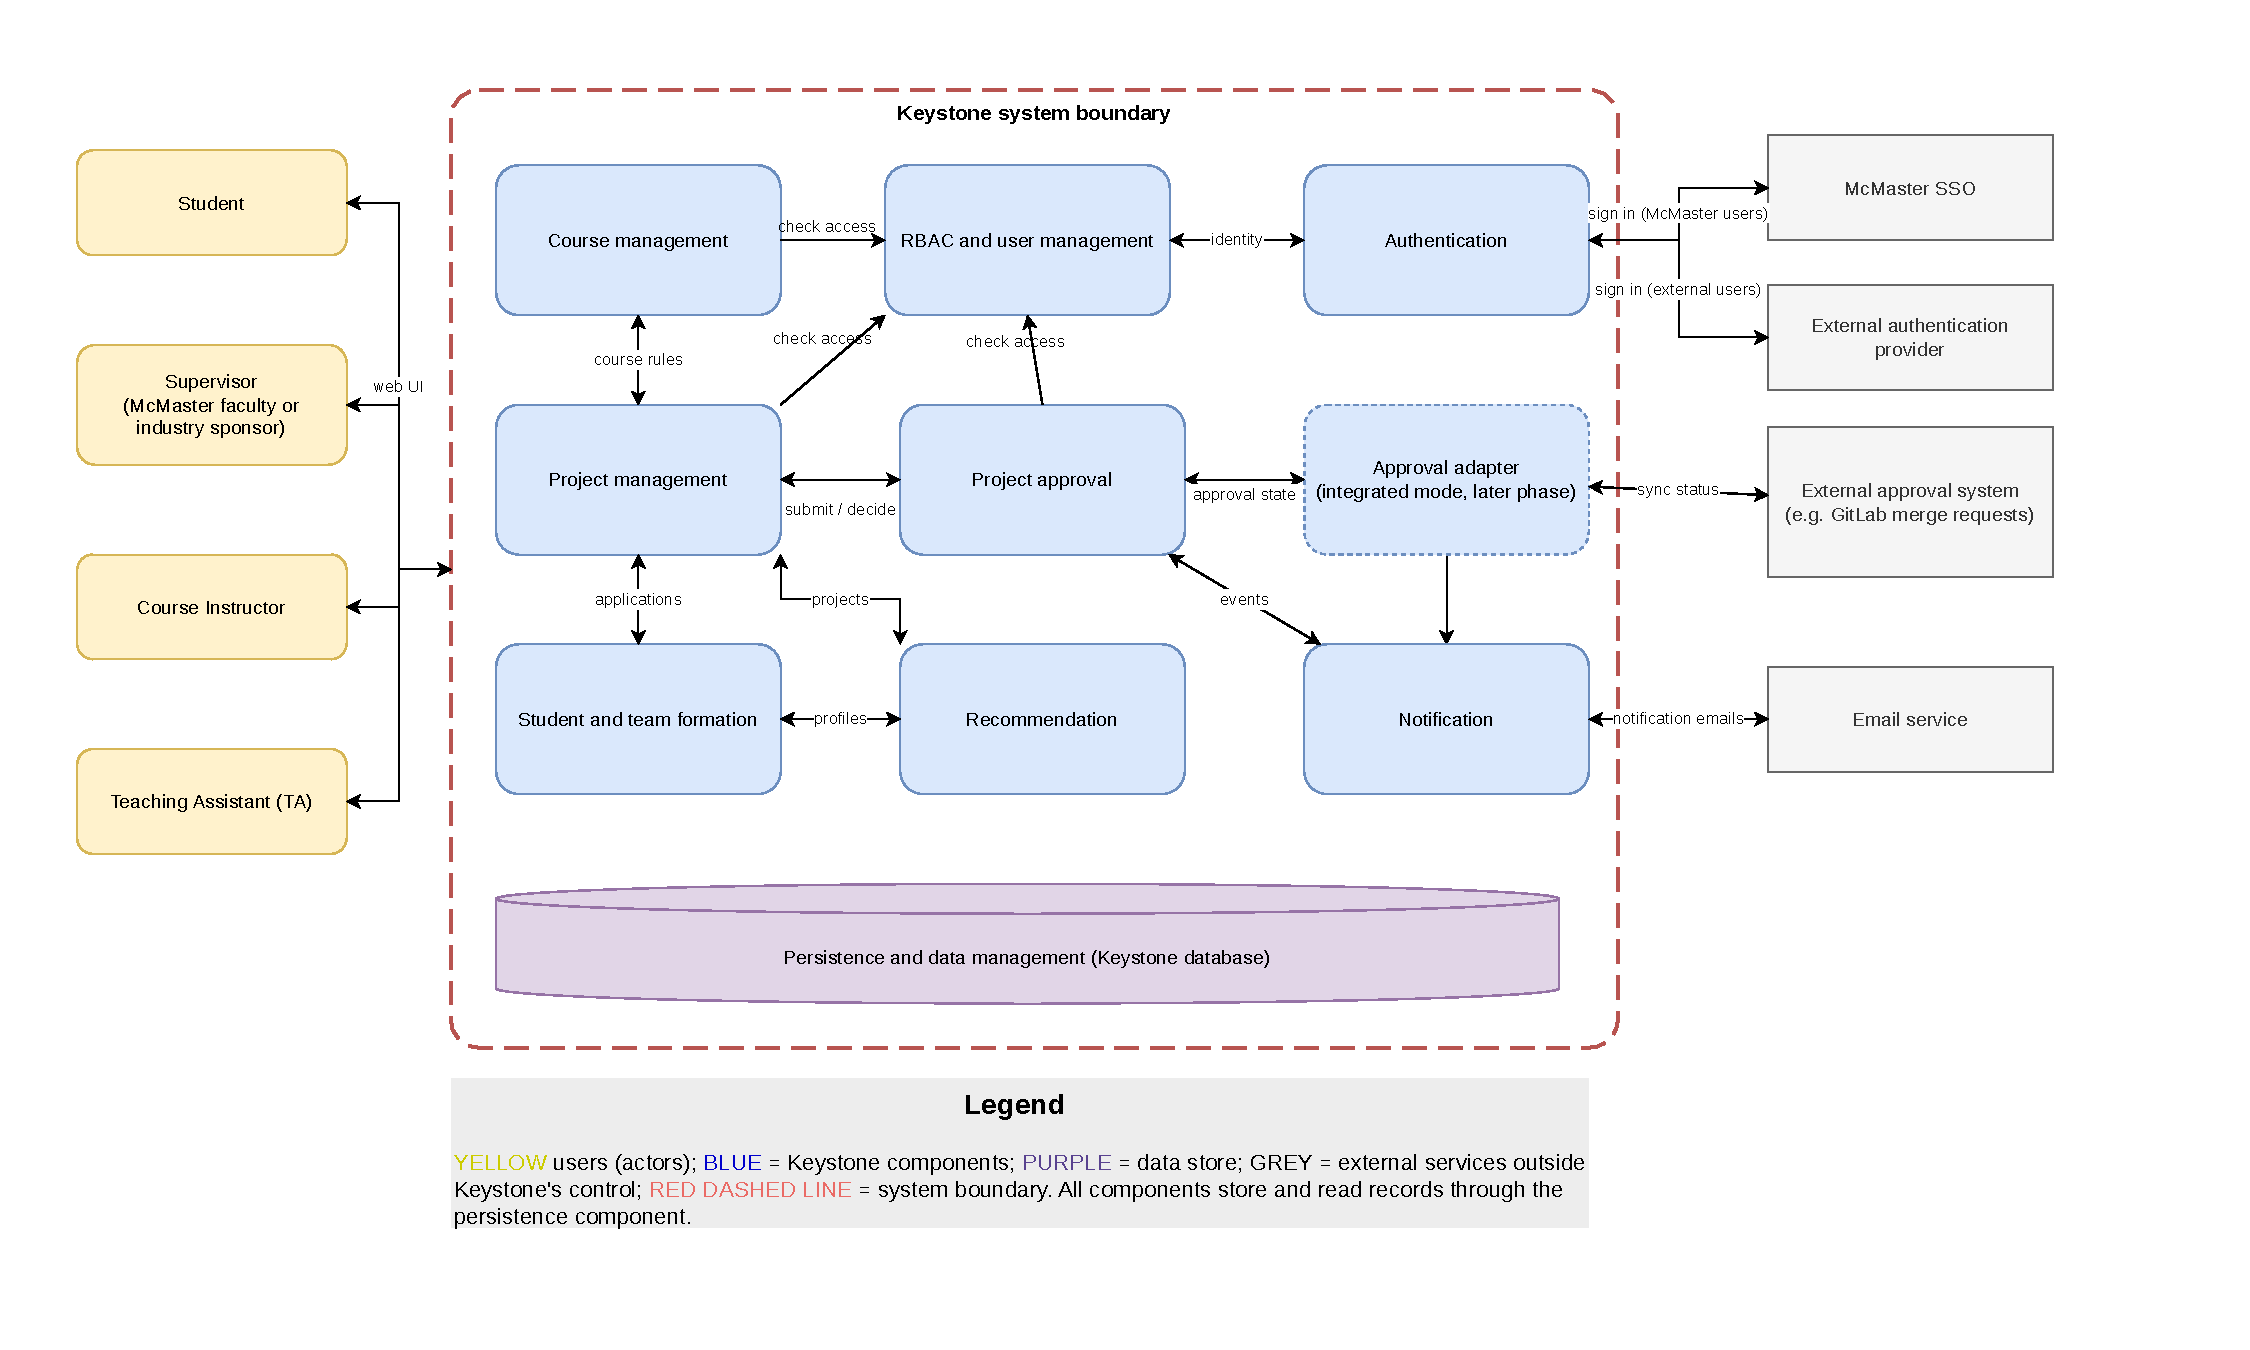
\includegraphics[width=\textwidth]{Keystone_SystemContext}
    \caption{System and boundary context diagram for \projname{}}\label{fig:systemcontext}
\end{figure}

The following external entities and services are relevant:

\begin{itemize}
    \item \textbf{McMaster single sign-on (SSO):}
    Provides authentication for users accessing \projname{}
    through their McMaster credentials.

    \item \textbf{External authentication provider:}
    Supports authentication for users who do not have a
    McMaster account.

    \item \textbf{Email service:}
    Delivers notifications concerning project submissions,
    approvals, supervisor confirmations, and other events.

    \item \textbf{External approval system:}
    A course-specific system outside \projname{} where a course approves team projects, for
    example the GitLab merge request process used by the Software Engineering course. It is
    not under \projname{}'s control. In \emph{external} approval mode, the instructor or a TA
    records the approval outcome in \projname{} by hand. In \emph{integrated} mode, an approval
    adapter (a \projname{} component) reads the approval state through the external approval system's interface and
    updates \projname{}'s records.

    \item \textbf{Avenue to Learn:}
    McMaster's learning management system. \projname{} reads a course's enrollment list from it, for courses that have an
    Avenue site. It is not under \projname{}'s control and may be unavailable, out of date, or incomplete.
\end{itemize}

\subsection{Major Components}

The following components define the principal areas in which failures will be investigated. They are meant to
be functional boundaries for hazard identification, rather than a complete software architecture.

\begin{enumerate}
    \item \textbf{Authentication component:}
    Manages user sign-in through McMaster SSO and an external authentication provider.
    It is responsible for establishing the identity associated
    with a user session. Authentication failures may allow
    unauthorized access or prevent legitimate users from
    accessing the platform.

    \item \textbf{Role-Based Access Control (RBAC) and
    user management component:}
    Maintains user accounts, roles, and permissions. It determines which resources users may view or modify.
    Relevant roles include students, supervisors, TAs, and course instructors. Incorrect permissions may expose
    restricted information or allow unauthorized changes.

    \item \textbf{Course management component:}
    Maintains course configurations, course membership, instructor and TA assignments, course-specific rules and
    configurations, and relevant deadlines or course information. It must accommodate differences between Software
    Engineering (SE), Computer Science (CS), and Mechatronics (TRON) courses.

    \item \textbf{Project management component:}
    Manages project proposals, descriptions, supervisors, contact details, project categories, confidentiality
    information, intellectual property (IP) concerns, repository links, and project status throughout the
    project lifecycle.

    \item \textbf{Project approval component:}
    Supports project proposal review, team project approval, and the recording of approval decisions. It must
    distinguish between submission, review, approval, and other workflow states so that users are not misled
    about whether a project or team has been approved.

    \item \textbf{Student and team formation component:}
    Manages student profiles, team membership, project interests, and any supported team or project
    recommendations. It must respect course eligibility rules and team-size constraints.

    \item \textbf{Notification component:}
    Generates and sends notifications associated with relevant workflow events via the email service.
    Failures may result in missing, delayed, duplicated, or incorrectly addressed messages.

    \item \textbf{Persistence and data management component:}
    Stores and retrieves the platform's persistent records.
    It maintains the consistency of related information,
    including project records, team membership, course
    configuration, approval states, and user permissions.

    \item \textbf{Approval adapter (integrated mode):}
    Reads approval state from an external approval system and updates \projname{}'s records.
    Failures may leave \projname{} showing a state that differs from the external system.

    \item \textbf{Recommendation component:}
    Ranks or filters projects and potential
    team matches based on available information and user
    preferences. Incorrect recommendations may hide
    relevant opportunities or mislead users about their
    suitability for a project.
\end{enumerate}

\section{Critical Assumptions}

\wss{These assumptions that are made about the software or system.  You should
minimize the number of assumptions that remove potential hazards.  For instance,
you could assume a part will never fail, but it is generally better to include
this potential failure mode.}


\begin{enumerate}
    \item \textbf{Instructor authority:}
        Course instructors remain responsible for final project
        approval, the interpretation of course rules, and
        exceptional team-formation decisions. \projname{} supports
        these decisions but does not replace the instructor's
        judgment regarding project feasibility, scope, or
        academic suitability.
    \item \textbf{Authentication provider availability:}
        McMaster SSO and any external authentication provider
        are external dependencies and may become unavailable.
        \projname{} cannot guarantee their continuous operation
        but must handle authentication failures safely.
    \item \textbf{Accuracy of user-supplied information:}
        Students and supervisors may submit incomplete,
        incorrect, misleading, or outdated information.
        The platform can validate information according to
        defined rules, but it cannot guarantee the truth of
        every project description, supervisor commitment, or
        user-provided statement.
    \item \textbf{Feature configuration:}
        Optional features may be disabled by course instructors
        to support different capstone courses or future
        deployments. Disabling a feature must not leave
        dependent workflows in an invalid state or expose
        information that would otherwise be restricted.
    \item \textbf{Enrollment data availability and accuracy:}
        Avenue to Learn is an external dependency, and not every course has an Avenue site. Its enrollment data may be
        unavailable, out of date, or incomplete. \projname{} cannot guarantee that an imported list is correct, so course
        staff remain responsible for confirming imports and for adding students who are missing.
\end{enumerate}

\setlength{\tabcolsep}{4pt}
\newlength{\fw}
\setlength{\fw}{\dimexpr\textheight-14\tabcolsep-12pt\relax}

\begin{landscape}

\section{Failure Mode and Effect Analysis}
\small
\renewcommand{\arraystretch}{1.15}

\wss{Include your FMEA table here. This is the most important part of this document.}
\wss{The safety requirements in the table do not have to have the prefix SR.
The most important thing is to show traceability to your SRS. You might trace to
requirements you have already written, or you might need to add new
requirements.}
\wss{If no safety requirement can be devised, other mitigation strategies can be
entered in the table, including strategies involving providing additional
documentation, and/or test cases.}

\begin{longtable}{
        >{\raggedright\arraybackslash}p{0.10\fw}
        >{\raggedright\arraybackslash}p{0.13\fw}
        >{\raggedright\arraybackslash}p{0.14\fw}
        >{\raggedright\arraybackslash}p{0.12\fw}
        >{\raggedright\arraybackslash}p{0.20\fw}
        >{\raggedright\arraybackslash}p{0.16\fw}
        >{\raggedright\arraybackslash}p{0.15\fw}}
\caption{Failure Mode and Effect Analysis}\label{tab:fmea}\\
\toprule
\textbf{Component} & \textbf{Failure Mode} & \textbf{Effects of Failure} & \textbf{Causes of Failure} & \textbf{Recommended Action} & \textbf{SR} & \textbf{Ref} \\
\midrule
\endfirsthead
\toprule
\textbf{Component} & \textbf{Failure Mode} & \textbf{Effects of Failure} & \textbf{Causes of Failure} & \textbf{Recommended Action} & \textbf{SR} & \textbf{Ref} \\
\midrule
\endhead
\midrule
\multicolumn{7}{r}{\emph{Continued on next page}} \\
\endfoot
\bottomrule
\endlastfoot

Authentication &
SSO or external provider unavailable &
Users cannot access platform, leads to missed deadlines &
External service outage, network failure &
Display error, log failure, raise warning to IT department and/or instructors &
\ssrref{SSR_ExternalErrorLogging} &
\reqitem{hnum}{H_AuthProviderOutage} \\

\addlinespace
\addlinespace

&
User session is stolen &
Attacker can act as the user, read sensitive data, perform unapproved actions &
Compromised device, unencrypted user traffic, compromised external service &
Re-verify the user before every action on the closed list in \ssrref{SSR_ReverifyCriticalActions} &
\ssrref{SSR_ReverifyCriticalActions} &
\reqitem{hnum}{H_SessionTheft} \\

\addlinespace
\hline
\addlinespace

RBAC and user management &
User is assigned the wrong role  &
Student able to act as a course instructor, supervisor as an IT technician, etc. &
System inferring roles from an unreliable source &
Default to zero privileges if automatic assignment fails, provide instructor with ability to modify roles, and record all actions in an audit log &
\ssrref{SSR_AuditLog}, \ssrref{SSR_ZeroDefaultPrivileges} &
\reqitem{hnum}{H_WrongRole} \\

\addlinespace
\addlinespace

&
A person with no connection to the course signs in through the external provider and is treated as a supervisor &
Student information and student-proposed projects are disclosed to outsiders, and the platform can be scraped &
The external provider accepts any identity, and the role is assigned at sign-in &
Give every external sign-in the unverified external supervisor role, limited to course reference material, the proposal template, and their own proposals, and verify it only when an instructor approves a proposal that the account submitted &
\ssrref{SSR_ExternalSupervisorVerification}, \ssrref{SSR_ZeroDefaultPrivileges} &
\reqitem{hnum}{H_UnvettedExternalAccess} \\

\addlinespace
\addlinespace

&
An external supervisor reads another sponsor's confidential project &
Loss of confidentiality of industry project ideas, loss of sponsor trust, IP disputes &
Visibility rules written for ``course members'' applied to all supervisors, or other sponsors' projects exposed through search, counts, status, or email &
Scope every read path for an external supervisor to the projects they proposed or are named on, and answer other requests as not found &
\ssrref{SSR_ExternalSupervisorScope}, \ssrref{SSR_EnforceVisibility} &
\reqitem{hnum}{H_CrossSponsorExposure} \\

\addlinespace
\hline
\addlinespace

Course management &
Disabling a feature leaves dependent workflows in an invalid state &
Other components fail unnecessarily and system rejects normal actions &
Component state does not account for all possible configurations &
Reject disable request, advise user on actions needed before feature can be disabled &
\ssrref{SSR_RejectDisable}, \ssrref{SSR_NotifyPendingActions} &
\reqitem{hnum}{H_DisableBreaksWorkflow} \\

\addlinespace
\addlinespace

&
Team formation rules are misconfigured, or changed after teams have formed &
Valid teams are blocked, or invalid teams are accepted; teams that were valid under the old rules become non-compliant without notice &
Wrong team size limits or program combinations entered, rule edits applied without checking existing teams &
Validate the rule configuration on save, restrict edits to instructors, preview the teams a change would make non-compliant, and flag those teams for instructor review instead of invalidating them &
\ssrref{SSR_RuleChangeImpact}, \ssrref{SSR_AuditLog} &
\reqitem{hnum}{H_RuleMisconfiguration} \\

\addlinespace
\hline
\addlinespace

Project management &
Project displays outdated information &
Teams operate based on false information, contacting individuals which may no longer be involved with the course &
Instructor, supervisor, or even students forget to update their information &
Display a timestamp for when any displayed records were last updated &
\ssrref{SSR_RecordTimestamps} &
\reqitem{hnum}{H_OutdatedProject} \\

\addlinespace
\addlinespace

&
Confidential project or IP exposed &
Potential monetary loss, loss of trust, exposed vulnerabilities &
Project visibility rules not being enforced across a project &
Check every way of reading a record (catalog, search, project detail, threads, emails, exports, recommendations)
on the server against the visibility matrix in the SRS &
\ssrref{SSR_EnforceVisibility} &
\reqitem{hnum}{H_ConfidentialExposure} \\

\addlinespace
\addlinespace

&
Project description misrepresents project &
Team cannot move forward with project, time wasted &
Project proposal prompt not asking for critical information  &
Require every attribute that the SRS data dictionary marks as Required and prompt for the optional ones &
\ssrref{SSR_ProposalPromptCoverage} &
\reqitem{hnum}{H_MisleadingDescription} \\

\addlinespace
\addlinespace

&
A supervisor accepts a team and takes the last slot, but the project is not shown as Full (or a released slot does not reopen it) &
Other teams apply to or wait on a project that cannot take them &
Failure between reserving the slot and updating the project status or notifying applicants &
Reserve the slot, update the project status, and queue notifications to teams with open applications in a single transaction &
\ssrref{SSR_AtomicActions} &
\reqitem{hnum}{H_StaleProjectStatus} \\

\addlinespace
\hline
\addlinespace

Project approval &
A team or supervisor sees ``Approved'' when the team-project status is Agreed, Submitted, or Under review, or a post-approval change replaces the approved record before the instructor accepts it &
Team acts on an approval it does not have, or the official record is wrong &
Displayed status derived separately from the stored status, change requests written directly to the approved record &
Display only the stored team-project status using the lifecycle labels, hold changes to an approved record as pending, and apply them only when the instructor accepts &
\ssrref{SSR_ApprovalStatusIntegrity} &
\reqitem{hnum}{H_MisleadingApprovalStatus} \\

\addlinespace
\hline
\addlinespace

Approval adapter (integrated mode) &
Synchronization with the external approval system is stale or fails &
\projname{} shows a status that differs from the external system, a team misses a deadline or is treated as approved or unapproved incorrectly &
External system outage or interface change, adapter error, delayed polling &
Show the time of the last successful sync on externally approved records, flag failed syncs, and let the instructor or TA record the outcome manually (logged) &
\ssrref{SSR_AdapterSyncStatus} &
\reqitem{hnum}{H_AdapterSyncFailure} \\

\addlinespace
\hline
\addlinespace

Student and team formation &
Two students attempt to join the last slot of a group simultaneously, neither receives a fail message &
Both students believe they have joined the group, team size limit may be exceeded due to the data race &
Database allows both operations to run concurrently without a locking mechanism &
Ensure that data entries that are part of a single operation are not modified externally for the total duration of the operation &
\ssrref{SSR_NoStaleReads} &
\reqitem{hnum}{H_TeamSizeRace} \\

Student and team formation &
Decline or rejection is communicated bluntly, or students feel publicly ranked &
Stress, feeling unfairly treated, students stop using the platform &
Free-text decline messages, visible statuses with no guidance &
Use respectful message templates with an optional reason, and show no public ranking of students or teams &
\ssrref{SSR_RespectfulDeclines} &
\reqitem{hnum}{H_BluntRejection} \\


\addlinespace
\hline
\addlinespace

Notification &
Important notification is not delivered &
User misses important deadline, fails to respond to time sensitive matter &
Notification component fails in the process of sending a notification, queued notification is lost &
Ensure that queued notifications remain available until delivery is verified to have completed &
\ssrref{SSR_DurableNotifications} &
\reqitem{hnum}{H_LostNotification} \\

\addlinespace
\addlinespace

&
Notification is sent to the wrong recipient &
Confidential proposal, IP, or student information is disclosed to someone who should not see it &
Recipients resolved from stale roles or associations, confidential fields placed in the email body &
Resolve recipients at send time from current role and association, and include only an event summary and a link in the email body &
\ssrref{SSR_NotificationRecipientScope} &
\reqitem{hnum}{H_MisaddressedNotification} \\

\addlinespace
\addlinespace

&
Same notification delivered more than once &
Users are confused or ignore later notifications, trust in the platform drops &
Retries after an unconfirmed delivery &
Give each notification a unique identifier so a retry never results in a second send &
\ssrref{SSR_NotificationDeduplication} &
\reqitem{hnum}{H_DuplicateNotification} \\

\addlinespace
\hline
\addlinespace

Persistence and data management &
Data is lost or corrupted &
User data is lost, system fails to operate as expected, audit log lost &
Hardware degradation, accidental deletion, migration failures &
Regular, automated backups which are verified to be able to restore platform to a previous, working state &
\ssrref{SSR_AutomatedBackups} &
\reqitem{hnum}{H_DataLoss} \\

&
Personal data kept longer than needed &
Privacy breach, loss of trust, legal exposure &
No retention policy, deletion not implemented &
Define a retention period and delete personal data on request and at the end of the course cycle &
\ssrref{SSR_PersonalDataDeletion} &
\reqitem{hnum}{H_ExcessRetention} \\

\addlinespace
\hline
\addlinespace

Recommendation &
Irrelevant projects ranked highly &
Users miss projects that interest them, due to the assumption that lower projects are not worth looking into &
Recommendation algorithm performs badly, inputs are outdated &
Provide multiple ways to sort project list &
\ssrref{SSR_MultipleBrowseViews} &
\reqitem{hnum}{H_IrrelevantRanking} \\

\addlinespace
\hline
\addlinespace

Enrollment import &
Avenue unavailable or the import fails &
Course cannot be populated with its students, team validation cannot run, team formation and approval are delayed &
Avenue outage, change to Avenue access, or the course has no Avenue site &
Leave existing enrollment unchanged, tell the user, and offer file upload &
\ssrref{SSR_EnrollmentFallback} &
\reqitem{hnum}{H_ImportUnavailable} \\

\addlinespace
\addlinespace

&
Import produces a wrong list (missing, duplicate, or mismatched students) &
Students wrongly blocked from or admitted to the course, invalid team validation results &
Stale or partial data from Avenue, malformed identifiers &
Check student identifiers, detect duplicates, and show an import preview for the user to review and confirm before applying changes. &
\ssrref{SSR_EnrollmentPreview}, \ssrref{SSR_EnrollmentValidation} &
\reqitem{hnum}{H_ImportWrongList} \\

\addlinespace
\addlinespace

&
Student missing from the import is removed from a team automatically &
Team becomes undersized or invalid in the middle of approval, student loses their place without notice &
Import treated as the single source of truth and applied without review &
Flag absent students for review and never remove them automatically &
\ssrref{SSR_NoAutoRemoval} &
\reqitem{hnum}{H_AutoRemovalFromTeam} \\

\addlinespace
\addlinespace

&
Student who joins late cannot be added &
Student has no team and no way to use the platform, and team formation is delayed &
The import is the only way to add students &
Let course staff add students from an additional file import &
\ssrref{SSR_EnrollmentFallback} &
\reqitem{hnum}{H_LateStudent} \\

\addlinespace

\end{longtable}
\end{landscape}

\section{Safety and Security Requirements}

\wss{Newly discovered requirements.  These should also be added to the SRS.  (A
rationale design process how and why to fake it.)}

\begin{itemize}
    \item[]\reqitem{ssrnum}{SSR_ExternalErrorLogging} The system shall log all errors caused by external providers and notify university IT professionals and/or course instructors when they are detected.\\
    \textbf{Rationale}: Outages caused by external providers prevent users from using the platform and require immediate attention to restore in a timely manner.\\
    \textbf{Fit Criterion}: An authorized administrator can read a log that contains external provider errors, and an instructor or IT contact is notified when one occurs.\\
    \textbf{Traces To}: \srsref{FR_LogExternalErrors}

    \item[]\reqitem{ssrnum}{SSR_AuditLog} The system shall record all user actions with the time, a user identifier, and their privilege level at the time of the action, in an append-only audit log.\\
    \textbf{Rationale}: Accounts may get compromised and any actions taken may need to be reviewed and reversed.\\
    \textbf{Fit Criterion}: One action of each type (approval decision, status change, role change) produces an entry with time, user identifier, and privilege level, and no interface or API path edits or deletes entries. \\
    \textbf{Traces To}: \srsref{NFR_AuditLog}, \srsref{NFR_AuditTamper}, \srsref{FR_AuthorizationRBAC}, \srsref{FR_UpdateRoles}

    \item[]\reqitem{ssrnum}{SSR_RejectDisable} The system shall reject all component disable requests if there are pending actions within the component.\\
    \textbf{Rationale}: Disabling features may potentially leave the system in a partially invalid state. For example, disabling the project approvals component strands pending project approval requests.\\
    \textbf{Fit Criterion}: Attempting to disable the project approval component while at least one approval record is pending is rejected, and the pending records are listed.\\
    \textbf{Traces To}: \srsref{FR_RejectComponentDisable}

    \item[]\reqitem{ssrnum}{SSR_RecordTimestamps} The system shall display a timestamp for any displayed records when they were last updated.\\
    \textbf{Rationale}: Providing users with a timestamp can allow them to judge whether the information they are reading is up-to-date and can contact instructors or supervisors when that is not the case.\\
    \textbf{Fit Criterion}: Every project and profile page displays a last-updated timestamp that changes when the record is modified.\\
    \textbf{Traces To}: \srsref{FR_DisplayTimestamps}

    \item[]\reqitem{ssrnum}{SSR_DurableNotifications} All pending notifications shall be stored durably until delivery is verified.\\
    \textbf{Rationale}: Lost notifications mean that users are not alerted of potentially time-sensitive matters and this can result in missed deadlines and loss of time.\\
    \textbf{Fit Criterion}: If the system is stopped before a queued notification is sent, the notification is sent after restart.\\
    \textbf{Traces To}: \srsref{FR_DurableNotifications}

    \item[]\reqitem{ssrnum}{SSR_AutomatedBackups} The platform shall provide a mechanism for automatically creating regular backups which can restore the platform to a previous state.\\
    \textbf{Rationale}: Data loss incidents are not uncommon and can be caused by faulty hardware, accidental changes, and many others. Storing a set of backups ensures that any data loss is minimized to a backup period timespan.\\
    \textbf{Fit Criterion}: Restoring the latest backup into a clean environment reproduces the project, team, and approval records.\\
    \textbf{Traces To}: \srsref{NFR_Recoverable}

    \item[]\reqitem{ssrnum}{SSR_MultipleBrowseViews} The platform shall provide multiple ways to find, filter, and browse the list of projects.\\
    \textbf{Rationale}: While a recommendation engine is proposed, it may be flawed or operate on outdated data. To ensure users don't miss a project that they may favour, providing multiple ways to display the list can bring different projects to the top.\\
    \textbf{Fit Criterion}: The catalog offers search, filters, and at least two sort orders, and every open project can be reached without using recommendations.\\
    \textbf{Traces To}: \srsref{FR_ViewApprovedProjects}

    \item[]\reqitem{ssrnum}{SSR_AtomicActions} All system actions which involve multiple dependent reads and writes, with at least one write, shall be atomic.\\
    \textbf{Rationale}: System actions which involve multiple steps may fail at any point, leaving the system in a partially corrupt state. Atomicity guarantees that an operation either fully completes, or fully fails. Operations which fail can then simply be retried.\\
    \textbf{Fit Criterion}: A fault injected after the first write of slot reservation, slot release, and approval leaves either all or none of that action's changes.\\
    \textbf{Traces To}: \srsref{NFR_ConcurrencySafety}

    \item[]\reqitem{ssrnum}{SSR_NoStaleReads} The system shall ensure that operations on sets or aggregations of multiple data entries do not operate on stale data at any point during an operation.\\
    \textbf{Rationale}: Concurrent operations which rely on aggregations of data entries may introduce a data race, resulting in an invalid state after the operation. For example, two students attempting to join the same team which only has one available slot can end up exceeding the team size limit, if the mechanism is not implemented correctly.\\
    \textbf{Fit Criterion}: Over repeated runs, two simultaneous requests to join a team with one free slot produce exactly one success and one explicit failure.\\
    \textbf{Traces To}: \srsref{NFR_ConcurrencySafety}

    \item[]\reqitem{ssrnum}{SSR_NotifyPendingActions} The system shall notify the user of pending actions when disabling a component fails.\\
    \textbf{Rationale}: It may be possible to disable certain components but require additional actions to be taken, such as responding to pending project approvals.\\
    \textbf{Fit Criterion}: Attempting to disable the project approval component while at least one approval record is pending is rejected, and the pending records are listed.\\
    \textbf{Traces To}: \srsref{FR_RejectComponentDisable}

    \item[]\reqitem{ssrnum}{SSR_ReverifyCriticalActions} The system shall re-verify the user before performing any of the following actions: (1) changing credentials, email, or linked authentication; (2) deleting a proposal, project, profile, thread, or account; (3) changing a user's role or course association; (4) a supervisor or team accepting an agreement; (5) leaving or dissolving a team; (6) a final instructor or TA approval or rejection; (7) confirming an enrollment import or changing course rules or the approval mode. This list is closed; adding an action requires amending this requirement. Re-verification must include at least one of: re-entering credentials, entering an email code, responding to an MFA challenge, and/or responding to an SSO challenge.\\
    \textbf{Rationale}: Sessions may get stolen or unsecured devices may get compromised. Actions which are difficult to undo should be protected to ensure the actual account holder is performing the action.\\
    \textbf{Traces To}: \srsref{FR_ReverifyUsers}\\
    \textbf{Fit Criterion}: For each of the seven actions, attempting it in a session that has not been re-verified prompts for re-verification and does not perform the action until it succeeds.

    \item[]\reqitem{ssrnum}{SSR_EnforceVisibility} The system shall check every way of reading a record on the server against the visibility matrix in \srsref{DPR_VisibilityMatrix}. The covered channels are the project catalog, search and filters, project detail pages, threads, notification emails, exported reports, and recommendations.\\
    \textbf{Rationale}: Exposing IP or confidential information can lead to damages and loss of trust. Checking only some channels leaves the others as a way around the restriction.\\
    \textbf{Traces To}: \srsref{FR_AuthorizationRBAC}, \srsref{DPR_VisibilityMatrix}, \srsref{DPR_RoleBasedDataPermissions}\\
    \textbf{Fit Criterion}: For each role and each covered channel, requesting a record that the matrix hides from that role is denied, and no notification email or export contains a field the recipient is not permitted to read.

    \item[]\reqitem{ssrnum}{SSR_ProposalPromptCoverage} The proposal template shall require every Project attribute that the SRS data dictionary (\srsref{FR_SupervisorProposal}) marks as Required (background, objectives, impact, completion status, industry, supervisor capacity, confidentiality, and IP) and shall prompt for the Optional attributes.\\
    \textbf{Rationale}: Prompting only an open-ended description gives supervisors no information on what students and instructors are looking for in a capstone-level project, and omits what students need to judge a project (for example how much already exists).\\
    \textbf{Traces To}: \srsref{FR_SupervisorProposal}, \srsref{FR_ProposalOptionalFields}\\
    \textbf{Fit Criterion}: Submission is blocked, with the empty field highlighted, if any Required attribute is empty, and succeeds when only Optional attributes are empty.

    \item[]\reqitem{ssrnum}{SSR_ZeroDefaultPrivileges} The system shall assign new users zero privileges when their identity cannot be assigned automatically or verified. The exception is a new sign-in through the external authentication provider, which is assigned the unverified external supervisor role.\\
    \textbf{Rationale}: No assumptions can be made about new users. They may be students who are not enrolled in a capstone course, malicious actors attempting to extract user information, individuals posing as supervisors to get free labour, etc. Ensuring no unverified users get access to student information mitigates those risks. Unverified external supervisors need only course reference material and their own proposals to submit a proposal.\\
    \textbf{Traces To}: \srsref{FR_MacSSO}, \srsref{FR_AuthorizationRBAC}, \srsref{FR_UpdateRoles}, \srsref{NFR_Authorize}, \srsref{FR_ExternalSupervisorVerification}\\
    \textbf{Fit Criterion}: A McMaster account with no assigned role receives an authorization error on every read and write of course data. A new external sign-in can read only course reference material, the proposal template, and its own proposals.

    \item[]\reqitem{ssrnum}{SSR_ExternalSupervisorVerification} The system shall give an external supervisor access to student profiles and student-proposed projects only after an instructor approves a project proposal that the external supervisor submitted, and shall record the verification in the audit log. No other action shall verify an external supervisor.\\
    \textbf{Rationale}: An external identity provider cannot confirm that a person is an industry sponsor, and student information must not be available to anyone who signs in. The instructor's review of a real proposal is the check.\\
    \textbf{Traces To}: \srsref{FR_ExternalSupervisorVerification}, \srsref{FR_UpdateRoles}\\
    \textbf{Fit Criterion}: A new external account requesting a student profile receives an authorization error. It can read one after an instructor approves its proposal, but not if a student proposal naming it is approved, and the verification appears in the audit log.

    \item[]\reqitem{ssrnum}{SSR_ExternalSupervisorScope} The system shall restrict an external supervisor, on every channel listed in \ssrref{SSR_EnforceVisibility}, to the access specified in the SRS (\srsref{FR_ExternalSupervisorScope}): unverified external supervisors to course reference material, the proposal template, and their own proposals, and verified ones additionally to student profiles, student-proposed projects, and the applications to their own projects. Requests for any other supervisor's proposal or project shall be answered as not found.\\
    \textbf{Rationale}: Industry project ideas are confidential, and any person can obtain an external account.\\
    \textbf{Traces To}: \srsref{FR_ExternalSupervisorScope}, \srsref{DPR_VisibilityMatrix}\\
    \textbf{Fit Criterion}: For each channel, an external supervisor requesting another sponsor's project receives a not-found response, and that project does not appear in any list, search result, count, or email to them. An unverified external supervisor is denied student profiles on every channel.

    \item[]\reqitem{ssrnum}{SSR_PersonalDataDeletion} The system shall delete personal data on request and at the end of a course cycle, and shall collect only the data that a feature needs. Audit log entries are retained, with the user reference anonymized.\\
    \textbf{Rationale}: Keeping personal data longer than needed increases the harm of a breach. Anonymizing rather than deleting audit entries keeps the audit log trustworthy.\\
    \textbf{Traces To}: \srsref{NFR_EssentialPersonal}, \srsref{DPR_UserManagedContentDeletion}, \srsref{DPR_EndOfTermStudentDataDeletion}, \srsref{DPR_ConsentWithdrawal}\\
    \textbf{Fit Criterion}: After a deletion request or the end-of-term job, personal fields are absent from the database and from exports (except data covered by consent to retain), and audit entries remain with no identifying user reference.

    \item[]\reqitem{ssrnum}{SSR_RespectfulDeclines} The system shall present decline and rejection decisions with respectful message templates and shall not publish rankings of students or teams.\\
    \textbf{Rationale}: Blunt or public decisions cause stress and a sense of unfair treatment, and may stop students from using the platform.\\
    \textbf{Fit Criterion}: Every decline or rejection message is generated from a template, and no page ranks students or teams.\\
    \textbf{Traces To}: \srsref{FR_DeclineTeam}

    \item[]\reqitem{ssrnum}{SSR_EnrollmentPreview} The system shall show a preview of any enrollment import and shall apply it only after course staff confirm it.\\
    \textbf{Rationale}: An unchecked import could wrongly add or exclude students and give misleading team validation results.\\
    \textbf{Fit Criterion}: An import changes no enrollment record until the user confirms the preview.\\
    \textbf{Traces To}: \srsref{FR_ImportEnrollment}

    \item[]\reqitem{ssrnum}{SSR_EnrollmentFallback} If an enrollment import fails or does not include a student, the system shall leave existing enrollment unchanged, tell the user, and let course staff add students from a file or manually.\\
    \textbf{Rationale}: Avenue may be unavailable, may not exist for a course, or may lack late-joining students, and course staff must still be able to populate the course.\\
    \textbf{Fit Criterion}: With Avenue unavailable, existing enrollment is unchanged, an error is shown, and file upload and manual add both work.\\
    \textbf{Traces To}: \srsref{FR_LogExternalErrors}, \srsref{FR_ImportEnrollment}, \srsref{FR_UpdateEnrollment}

    \item[]\reqitem{ssrnum}{SSR_NoAutoRemoval} The system shall not remove a student from a course or team because the student is absent from an enrollment import, and shall flag such students for confirmation by course staff.\\
    \textbf{Rationale}: Automatic removal could leave a team undersized or invalid in the middle of approval.\\
    \textbf{Fit Criterion}: A student on a team who is absent from the latest import stays on the team and appears on a review list.\\
    \textbf{Traces To}: \srsref{FR_EnrollmentDiscrepency}

    \item[]\reqitem{ssrnum}{SSR_EnrollmentValidation} The system shall check imported enrollment for duplicate and malformed student entries and show any problems in the preview before the import can be confirmed.\\
    \textbf{Rationale}: Stale or partial data from an external source can corrupt enrollment records.\\
    \textbf{Fit Criterion}: Duplicate and malformed entries are listed in the preview and block confirmation until resolved.\\
    \textbf{Traces To}: \srsref{FR_ImportEnrollment}

    \item[]\reqitem{ssrnum}{SSR_ApprovalStatusIntegrity} The system shall display team-project status only from the stored status, using the lifecycle labels in the SRS, and shall hold a change to an approved record as pending until the instructor accepts it.\\
    \textbf{Rationale}: Users act on the status they see. Showing Approved before approval, or altering the approved record early, leads teams and supervisors to act on an approval that does not exist.\\
    \textbf{Traces To}: \srsref{FR_ViewProjectStatus}, \srsref{FR_ApprovalRevision}, \srsref{FR_RequestApproval}\\
    \textbf{Fit Criterion}: A team in each non-Approved status is never displayed as Approved, and a submitted change to an approved record leaves the approved values unchanged until the instructor accepts it.

    \item[]\reqitem{ssrnum}{SSR_AdapterSyncStatus} For records whose approval comes from an external approval system, the system shall show the time of the last successful synchronization, flag a failed synchronization, and allow the instructor or TA to record the outcome manually, with the manual change logged.\\
    \textbf{Rationale}: A stale or failed sync makes \projname{} disagree with the system that holds the real decision, and users need to see that the data may be out of date.\\
    \textbf{Traces To}: \srsref{FR_ExternalApproval}\\
    \textbf{Fit Criterion}: With the external system made unavailable, the record shows the last-synced time and a failure flag, and a manual override by course staff is saved with an audit entry.

    \item[]\reqitem{ssrnum}{SSR_NotificationRecipientScope} The system shall determine each notification's recipients at send time from the user's current role and association with the item, and shall limit the email body to an event summary and a link, excluding confidential project, IP, and profile fields.\\
    \textbf{Rationale}: A misaddressed email can disclose confidential information outside the platform, where visibility rules cannot be enforced.\\
    \textbf{Traces To}: \srsref{FR_ThreadsNotify}, \srsref{DPR_PreventUnauthorizedDisclosure}\\
    \textbf{Fit Criterion}: After a user's role or association with an item is removed, no further notifications for that item are sent to them, and sampled emails contain no confidential fields.

    \item[]\reqitem{ssrnum}{SSR_NotificationDeduplication} The system shall give each notification a unique identifier and shall not send the same notification to the same recipient more than once, including when delivery is retried.\\
    \textbf{Rationale}: Durable delivery retries until success, which can duplicate messages if a confirmation is lost.\\
    \textbf{Traces To}: \srsref{FR_DurableNotifications}\\
    \textbf{Fit Criterion}: When delivery confirmation is suppressed and delivery retried, the recipient receives the notification exactly once.

    \item[]\reqitem{ssrnum}{SSR_RuleChangeImpact} The system shall validate the course team formation rules on save (minimum size at most maximum size, at least one permitted program combination), restrict editing them to instructors, show the teams that a change would make non-compliant before it is applied, and flag those teams for instructor review rather than invalidating them.\\
    \textbf{Rationale}: Wrong or retroactive rules can block valid teams or silently invalidate teams in the middle of approval.\\
    \textbf{Traces To}: \srsref{FR_ValidateTeamRules}, \srsref{FR_DisableFeatures}\\
    \textbf{Fit Criterion}: A configuration with minimum above maximum is rejected, a change that affects existing teams shows them in a preview, and after applying it those teams remain intact and appear on a review list.
\end{itemize}

\section{Roadmap}

\wss{Which safety requirements will be implemented as part of the capstone timeline?
Which requirements will be implemented in the future?}

The safety and security requirements follow the phases of the development plan in the SRS. A requirement is
implemented in the same phase as the feature it protects, so that no feature is released without the
protection that its hazards call for. Requirements that protect features outside the course timeline, or that
depend on parts of the system that are faked for the demo, are future work.

Within a phase, the order of requirements follows the dependencies between features in the SRS development plan,
not a computed risk score. Any requirement deferred to future work is listed below with the reason it can safely wait.

\subsection{Phase 1: Core Workflow (implemented in the course)}

Phase~1 covers proposal submission and approval, browsing projects with a visible status and team selection,
team project submission and review, and the validated team composition export.

\begin{itemize}
    \item \ssrref{SSR_ProposalPromptCoverage}: the proposal template asks for the information that makes a project viable as a capstone
    project (\hazref{H_MisleadingDescription}).
    \item \ssrref{SSR_EnforceVisibility}: server-side visibility checks for proposals and projects, tested for each role (\hazref{H_ConfidentialExposure}).
    \item \ssrref{SSR_ZeroDefaultPrivileges}: new accounts have no privileges until their role is assigned (\hazref{H_WrongRole}).
    \item \ssrref{SSR_AuditLog}: an append-only audit log for approval decisions, status changes, and role changes (\hazref{H_WrongRole}).
    Logging every user action is future work.
    \item \ssrref{SSR_ExternalSupervisorVerification}, \ssrref{SSR_ExternalSupervisorScope}: the unverified state for every external sign-in, verification through approval of the supervisor's own proposal, and external-supervisor scoping on every read path (\hazref{H_UnvettedExternalAccess}, \hazref{H_CrossSponsorExposure}). These stay in scope even though the demo uses simplified sign-in, because the role checks do not depend on the real identity provider.
    \item \ssrref{SSR_RecordTimestamps}: last-updated time shown on project records (\hazref{H_OutdatedProject}).
    \item \ssrref{SSR_MultipleBrowseViews}: several ways to sort and filter the project list when browsing (\hazref{H_IrrelevantRanking}). Ranked recommendations
    themselves are future work.
    \item \ssrref{SSR_AtomicActions}, \ssrref{SSR_NoStaleReads}: database transactions and locking for team selection, approvals, and team
    membership (\hazref{H_StaleProjectStatus}, \hazref{H_TeamSizeRace}).
    \item \ssrref{SSR_ExternalErrorLogging}: logging of errors from external providers (\hazref{H_AuthProviderOutage}). Notifying instructors by email is added with
    notifications in Phase~2.
    \item \ssrref{SSR_AutomatedBackups}: automated database backups by the hosting provider, and a restore test before release
    (\hazref{H_DataLoss}).
    \item \ssrref{SSR_RespectfulDeclines}: decline and rejection message templates, with no public rankings (\hazref{H_BluntRejection}).
    \item \ssrref{SSR_EnrollmentPreview}, \ssrref{SSR_EnrollmentFallback}, \ssrref{SSR_NoAutoRemoval}, \ssrref{SSR_EnrollmentValidation}: preview and confirmation, fallbacks, flagging, and
    checks for imported enrollment (\hazref{H_ImportUnavailable} to \hazref{H_LateStudent}). Enrollment import is part of Phase~1 in the SRS.
    \item \ssrref{SSR_ApprovalStatusIntegrity}: only the stored team-project status is displayed, and changes to approved records are held until accepted (\hazref{H_MisleadingApprovalStatus}).
    \item \ssrref{SSR_RuleChangeImpact}: validation of course rules and a preview of affected teams before a rule change is applied (\hazref{H_RuleMisconfiguration}).
\end{itemize}

\subsection{Phase 2: Communication and Visibility (implemented in the course)}

Phase~2 adds notifications and the checklist, team profiles and contact details, the course schedule, and
identifying unselected projects.

\begin{itemize}
    \item \ssrref{SSR_DurableNotifications}: pending notifications are stored in the database until delivery is confirmed, with retries
    (\hazref{H_LostNotification}).
    \item \ssrref{SSR_ExternalErrorLogging}: alerts to the instructor when an external provider fails (\hazref{H_AuthProviderOutage}).
    \item \ssrref{SSR_EnforceVisibility}: visibility checks are extended to team profiles, contact details, and unselected projects
    (\hazref{H_ConfidentialExposure}).
    \item \ssrref{SSR_NotificationRecipientScope}, \ssrref{SSR_NotificationDeduplication}: recipients resolved at send time, summary-only email bodies, and unique notification identifiers (\hazref{H_MisaddressedNotification}, \hazref{H_DuplicateNotification}).
\end{itemize}

\subsection{Phase 3: Extended Features (implemented if time allows)}

\begin{itemize}
    \item \ssrref{SSR_ProposalPromptCoverage}: the proposal prompts are extended to student-initiated proposals, with the guidelines and
    examples that this phase adds (\hazref{H_MisleadingDescription}).
    \item \ssrref{SSR_AtomicActions}, \ssrref{SSR_NoStaleReads}: the same locking and transactions are applied to supervisor capacity limits
    (\hazref{H_StaleProjectStatus}, \hazref{H_TeamSizeRace}).
\end{itemize}

\subsection{Future Work (not implemented, or faked for the demo)}

\begin{itemize}
    \item \ssrref{SSR_RejectDisable}, \ssrref{SSR_NotifyPendingActions}: rules for disabling components apply once features can be switched on and off for
    each course (modularity and other courses). Until then the hazard (\hazref{H_DisableBreaksWorkflow}) cannot occur.
    \item \ssrref{SSR_ReverifyCriticalActions}: re-verification with email codes or MFA depends on real authentication
    (McMaster accounts and external accounts), which is simplified for the demo. In the course the system only asks
    for confirmation before the destructive actions on the list (\hazref{H_SessionTheft}). The deferral is acceptable because demo accounts hold no real student or sponsor data.
    \item \ssrref{SSR_AdapterSyncStatus}: needed only when an adapter to an external approval system is built. Until then approvals are recorded manually, which is the case this requirement's manual override already covers (\hazref{H_AdapterSyncFailure}).
    \item \ssrref{SSR_MultipleBrowseViews}: ranking and explaining recommendations, with matching of teams to projects (\hazref{H_IrrelevantRanking}). The Phase~1 sorting and filtering already keep every project reachable without recommendations.
    \item \ssrref{SSR_AuditLog}: full action logging and tamper-evident storage. Phase~1 logs the actions whose outcomes may need review or reversal (approvals, status changes, role changes); logging every other action adds volume without supporting a decision.
    \item \ssrref{SSR_ExternalErrorLogging}: notifying university IT of provider outages. In the course deployment the instructor is notified in Phase~2; contacting IT depends on a hosting arrangement outside the course.
    \item \ssrref{SSR_PersonalDataDeletion}: deletion on request and at the end of a course cycle (\hazref{H_ExcessRetention}). The demo uses seeded data and holds no real student information, so retention harm arises only once a real deployment stores it. Minimal collection (\srsref{NFR_EssentialPersonal}) applies from Phase~1.
    \item Hazards of any integration with an external approval system beyond \hazref{H_AdapterSyncFailure} need requirements of their own when it is built.
\end{itemize}

\newpage{}

\section{Appendix --- Generative AI Use Disclosure}

\wss{ChatGPT (version 5) was used to brainstorm ideas for the template for this disclose section.}

Used Claude Sonnet 5.5 for the following,
  \noindent \begin{itemize}
    \item Asked it what are the common security risks apps face that collect profile data to come up with some ideas and reinforce some of my own.
    \item Used it to get more research into how data breaches can happen as well as data leaks.
    \item To draft a latex template for the FMEA table.
    \item Used it to check both documents against the checklist and rubric and
          asked it to flag anything that was missing and any grammar issues
  \end{itemize}


\subsection*{Verification of AI-Generated Content}
The team reviewed every AI-assisted passage before including it. References were checked against the
publisher or standards body listing. The FMEA rows, requirements and roadmap were checked by the team against
the SRS, including each requirement name in the ``Traces To'' lines. The team is responsible for the accuracy,
completeness, and consistency of this document.


\newpage{}

\section{Appendix --- Reflection}

\wss{Not required for CAS 741}

\input{../Reflection.text}

Waqar:
\begin{enumerate}
    \item What went well while writing this deliverable?
    During this deliverable, distributing work was very straightforward as there
    was a lot of work, but it was separable by section. It was all work we have
    seen before in prior courses with documentation, so it was very intuitive to
    write and come up with solutions/answers.

    \item What pain points did you experience during this deliverable, and how
    did you resolve them?
    During this deliverable, everyone was very busy because we had midterms and
    a lot of assignments due alongside this report. Sometimes it also became
    difficult to stay updated with everyone's parts. However, because we planned
    out our schedule well in advance, we were able to finish everything on time
    while also completing our other work. Everyone also posted updates in our
    team chat when they got the chance, so we all stayed in the loop.

    \item Which of your listed risks had your team thought of before this
    deliverable, and which did you think of while doing this deliverable? For
    the latter ones (ones you thought of while doing the Hazard Analysis), how
    did they come about?
    Before this deliverable we had thought about things like security issues or
    our app crashing, which would cause downtime. While working on the hazards,
    we came up with how a bug could lead to incorrect decisions being made in the
    actual workflow of our app, which would be chaotic. We also came up with the
    idea of security regarding the profiles of each person, as we wanted to
    collect some information to help supervisors get a better idea of who they
    are working with (the students).

    \item Other than the risk of physical harm (some projects may not have any
    appreciable risks of this form), list at least 2 other types of risk in
    software products. Why are they important to consider?
    First, data leakage is always a concern with any software product. It drives
    whether users can trust the developers. If we have a leak, how we handle it
    and what measures we take to prevent it show users that we want to protect
    them and that using the app is safe. Second, availability matters because the
    system handles time-sensitive information such as deadlines. We want the
    greatest uptime we can achieve so users do not have to worry about the app
    going down. Lastly, data correctness is important: while we are handling PII,
    we want to process it correctly and avoid sharing it with third parties
    without user consent.
\end{enumerate}

Ayush:
\begin{enumerate}
    \item What went well while writing this deliverable?

    A great part about this document is it really made us think about our project from a different
    perspective. It made us think about all the ways things could go wrong, maybe an external service failed,
    maybe a user did something wrong. It made us think about making our design more robust so it can handle external
    failures.
    It also made us think about internal system failures that could have drastic impacts on functionality, such as RBAC
    not working properly and data integrity concerns.
    Overall, it was actually quite intuitive to write this deliverable.

    \item What pain points did you experience during this deliverable, and how
    did you resolve them?
    The main issues with this deliverable were related to keeping everything consistent with the hazard analysis
    and the SRS. The scope of the system outlined in the SRS dictates the scope of the HA. The hazards and mitigation
    strategies outlined in the FMEA table must map directly to either functional, non-functional or data requirements
    in the SRS. But because everything is constantly changing while we are writing it, it was quite difficult to
    make sure both documents aligned.

    \item Which of your listed risks had your team thought of before this
    deliverable, and which did you think of while doing this deliverable? For
    the latter ones (ones you thought of while doing the Hazard Analysis), how
    did they come about?

    Going in, we mostly had the obvious software risks in our heads.
    We knew that login and permissions (SSO, external accounts, who can see what) could go wrong.
    We also worried about privacy via student profiles leaking, and supervisors’ or students’ project ideas getting “stolen”.
    And we knew that if the platform broke, team formation and approvals would get delayed.

    Most of the more specific risks only showed up once we went component by component through the FMEA.
    For example, we only thought about hurt feelings and fairness when we went through the HA slides and checklist.
    Additionally, we had not thought about data retention policies until we properly analyzed the persistence module.

    \item Other than the risk of physical harm (some projects may not have any
    appreciable risks of this form), list at least 2 other types of risk in
    software products. Why are they important to consider?

    One risk is security and privacy risk.
    This covers things like someone getting into an account they shouldn’t, or personal info and
    confidential project ideas leaking. It matters because people trust the platform with their data,
    and once that trust is gone they stop using it. There can also be legal consequences,
    since software systems have to follow privacy law.

    Psychological and social risk is a big risk in software systems.
    This is stress, embarrassment, feeling unfairly treated or excluded by how the software behaves.
    It matters because software shapes how people feel about a process. Something like a blunt rejection message
    or a visible ranking can really hurt someone, even though nothing “broke".

\end{enumerate}

Ahmed:
\begin{enumerate}
    \item What went well while writing this deliverable?

    Discovering new requirements which would have been, at best, implicit, really highlighted the value of a hazard analysis. Additionally, it also revealed that some hazards, such as storing invalid states, span multiple components and may require adjusting whole system architecture to completely mitigate.

    \item What pain points did you experience during this deliverable, and how
    did you resolve them?

    It was difficult accounting for all hazards, because of the complexity of the system as represented by its current requirements. The system needs to be modular, secure, maintain data integrity, provide administrator controls, among many others, which, not only have potential hazards within each component, but also raise potential hazards between components. For example, any networked component which does not reject unsecured connections compromises the entire system.

    \item Which of your listed risks had your team thought of before this
    deliverable, and which did you think of while doing this deliverable? For
    the latter ones (ones you thought of while doing the Hazard Analysis), how
    did they come about?

    Data security was a clear risk since the platform's most essential data to store and display is sensitive information such as student information, project ideas which may be intellectual property, etc.
    
    A non-obvious risk which was only raised during the hazard analysis was the data integrity hazard. Two students attempting to join the same team at the same time can end up corrupting the state of the system if not enough care is taken.

    \item Other than the risk of physical harm (some projects may not have any
    appreciable risks of this form), list at least 2 other types of risk in
    software products. Why are they important to consider?

    Data corruption risk is very real and plagues many production applications and can arise due to improper data handling. Data corruption is important to pay attention to because it's often silent and can be unrecoverable if the system does not have any recoverability mechanisms, which require prior planning.

    Another important risk to consider in software products is the user interface aspect. User interfaces which are not intuitive, require manuals or training to understand, or do not account for accessibility requirements, often discourage users from the platform and on a large scale, this can lead to the platform failing completely.

\end{enumerate}

Andrew:
\begin{enumerate}
    \item What went well while writing this deliverable?
    What went well while writing this deliverable was the learning experience of thinking about a Hazard Analysis
    for the first time. It was interesting to take a more critical approach when analyzing our project
    from a requirements perspective. I learned that it is important to understand what things could go 
    wrong with your project including project discovery failures, misuse and security breaches, incorrect
    functionality, and loss of data. Identifying these will help us build a security and hazard-free system.

    \item What pain points did you experience during this deliverable, and how
    did you resolve them?
    The main pain points with this document was that it was very new to us. It is initially difficult to 
    distinguish the content in here with what is already in the SRS. It was also a struggle finding 
    hazards since our system is not safety-critical. At the same time, it was also difficult to tell
    what information we needed to collect first (including in the SRS) before we analyzed the
    hazard categories.

    \item Which of your listed risks had your team thought of before this
    deliverable, and which did you think of while doing this deliverable? For
    the latter ones (ones you thought of while doing the Hazard Analysis), how
    did they come about?
    From the listed risks, we had already thought of security breaches, loss of privacy, and loss of data. We were able to think
    of these based on our own experiences as full-stack developers. One of the most important things in an 
    application is how its data will be handled. We have all heard of many stories about big companies that
    went through major issues when it came to their data disclosure and 3rd party access. We knew that securing our
    clients' data would be of utmost priority since there is sensitive information that users would want to keep securely stored.     

    \item Other than the risk of physical harm (some projects may not have any
    appreciable risks of this form), list at least 2 other types of risk in
    software products. Why are they important to consider?
    1. Loss or corruption of project information: They include failed updates or inconsistent records related to user information,
    project data, or selected documentation. When stakeholders use our product, they expect that our system retains their
    records securely. If their project, team, and profile related data is corrupted, the system becomes unusable.
    2. Disclosure or misuse: If any data leaks were to occur, personal information and any communications that users may have
    had through the system would become public. This exposure is undesired and could lead to serious confidentiality and privacy concerns.


\end{enumerate}

\bibliographystyle {plainnat}
\bibliography {../../refs/References}

\end{document}